\chapter{Experiment Design and Analysis}
\label{ch:ExperimentDesign}
This chapter introduces three Zorro validation studies: a pilot study,
a case study with students from the software engineering class as
participants, and an external collaborative case study with the TDD
community of developers and researchers. Zorro uses low-level software
development activity data to infer developer's TDD behaviors.  In
order to validate its capabilities of data collection and TDD behavior
inference, a secondary data source must be used. In my dissertation
research, I will introduce two ways to provide the secondary data:
recording individual developer's TDD development process using the
Eclipse Screen Recorder (ESR) \cite{esr}; and gathering developer's
feedback to their TDD behavior inference results using the Zorro
validation wizard.  I have already used the ESR approach in the pilot
study. In the second case study, I will plan to use both approaches.

\section{Zorro Validation Pilot Study}
In January 2006, we ran a pilot study at the University of Hawaii in
order to assess how well Zorro infers TDD development process using
the rule-based system. We found that Zorro accurately recognized
participants' TDD behaviors in a simple environment setting.

\subsection{Purpose of the Study}
There were two purposes for this study. One was to test whether Zorro 
could collect enough development activity data for TDD development 
behavior inference. The other was to test whether Zorro could 
recognize the actual TDD development behaviors using rule-based 
approach.

\subsection{Research Questions}
In the pilot study, I wanted to test the correctness of Zorro's
methodology for inferring developer's TDD behaviors. In order to
test this, I developed the Eclipse Screen Recorder \cite{esr} to
do field participant observation. Ad addition, I also wanted to 
test the capability of ESR to support Zorro validation. The specific 
research questions for the pilot study were:
\begin{itemize}
 \item Q1a: Does Zorro collect enough low-level development activities to
   infer developer's TDD behaviors?
 \item Q1b: Does Zorro's inference of TDD agree with analyses based upon
   participant observation?
 \item Q1c: Is ESR a suitable tool for Zorro validation study?
\end{itemize}

\subsection{Research Methodology and Design}

\subsubsection{Participants}
The participants in this pilot study were experienced Java programmers
who knew unit testing well. I recruited 7 volunteers who were interested
in TDD and were willing to participate this study.

\subsubsection{Design and Experimental Manipulation}
This study used a pre-experimental design called the one-shot case
study \cite{Creswell:03}. The treatment in this study was TDD. Every
participant developed a small program that simulated a stack data
structure in Java using the Eclipse IDE and TDD. Before the study 
started, we introduced the red/green/refactor principle of TDD to 
the participants if they did not know TDD before. The TDD rhythm 
\cite{TDDRhythm}, TDD quick reference guide \cite{TDDQuickReference}
and the step-wise stack TDD implementation instructions were three 
supplemental material to help participates program in TDD. ESR
was used in this study to record the development process for participant
observation.

\subsubsection{Instruments}
The IDE for this study is Eclipse. I instrumented participants' TDD
development processes with the Hackystat Eclipse Sensor and ESR.

\subsubsection{Procedure}

\begin{enumerate}
\item{Setup} 

The participants worked on their own computers or on a lab computer 
we provided. Prior to the study we confirmed that the lab computer 
had the following software installed: 
  \begin{itemize}
    \item JDK 
    \item Eclipse IDE 
    \item Hackystat Eclipse Sensor \cite{HackystatSensorInstallation:06}
    \item Eclipse Screen Recorder \cite{esr}
  \end{itemize}
When participants chose to work at home on their own computer, we
asked them to configure these software before participating this 
study.

\item{Introduction to TDD}

When participants did not have prior knowledge of TDD, we briefly
introduced TDD to them using Beck's simple TDD abstraction: the 
red/green/refactor order of programming. 

\item{Development in the Lab or at Home} 

Stack is a well-known problem that works according to the 
Last-In-First-Out (LIFO) principle. Participants in this study developed solutions to the stack
problem using TDD method. We provided them with three documents: the
graphic illustration of TDD rhythm, the TDD reference guide, and the
user stories of stack with TDD implementation instructions at Appendix
\ref{app:PilotStudyMaterial}.

\end{enumerate}

\subsection{Data Collection} 

The Hackystat Eclipse sensor collected and sent development activities
to the remote Hackystat server. I collected the programming videos
recorded by ESR using memory sticks for study conducted in the lab and
email attachments for study conducted by participants themselves at
home. 

\subsection{Data Analyses and Results}
\subsubsection{Inferring Participants' TDD Behavior Inference}
The Hackystat Eclipse sensor collected low-level development
activities and sent them to a Hackystat server. For each participant,
I defined a Hackystat project and inferred their TDD behaviors with
Zorro. Figure \ref{fig:gui} is a Zorro inference report example using my 
own data. It displays both low-level development activity data used 
for TDD inference and the inferred results. 
\begin{figure}[htbp]
  \centering
  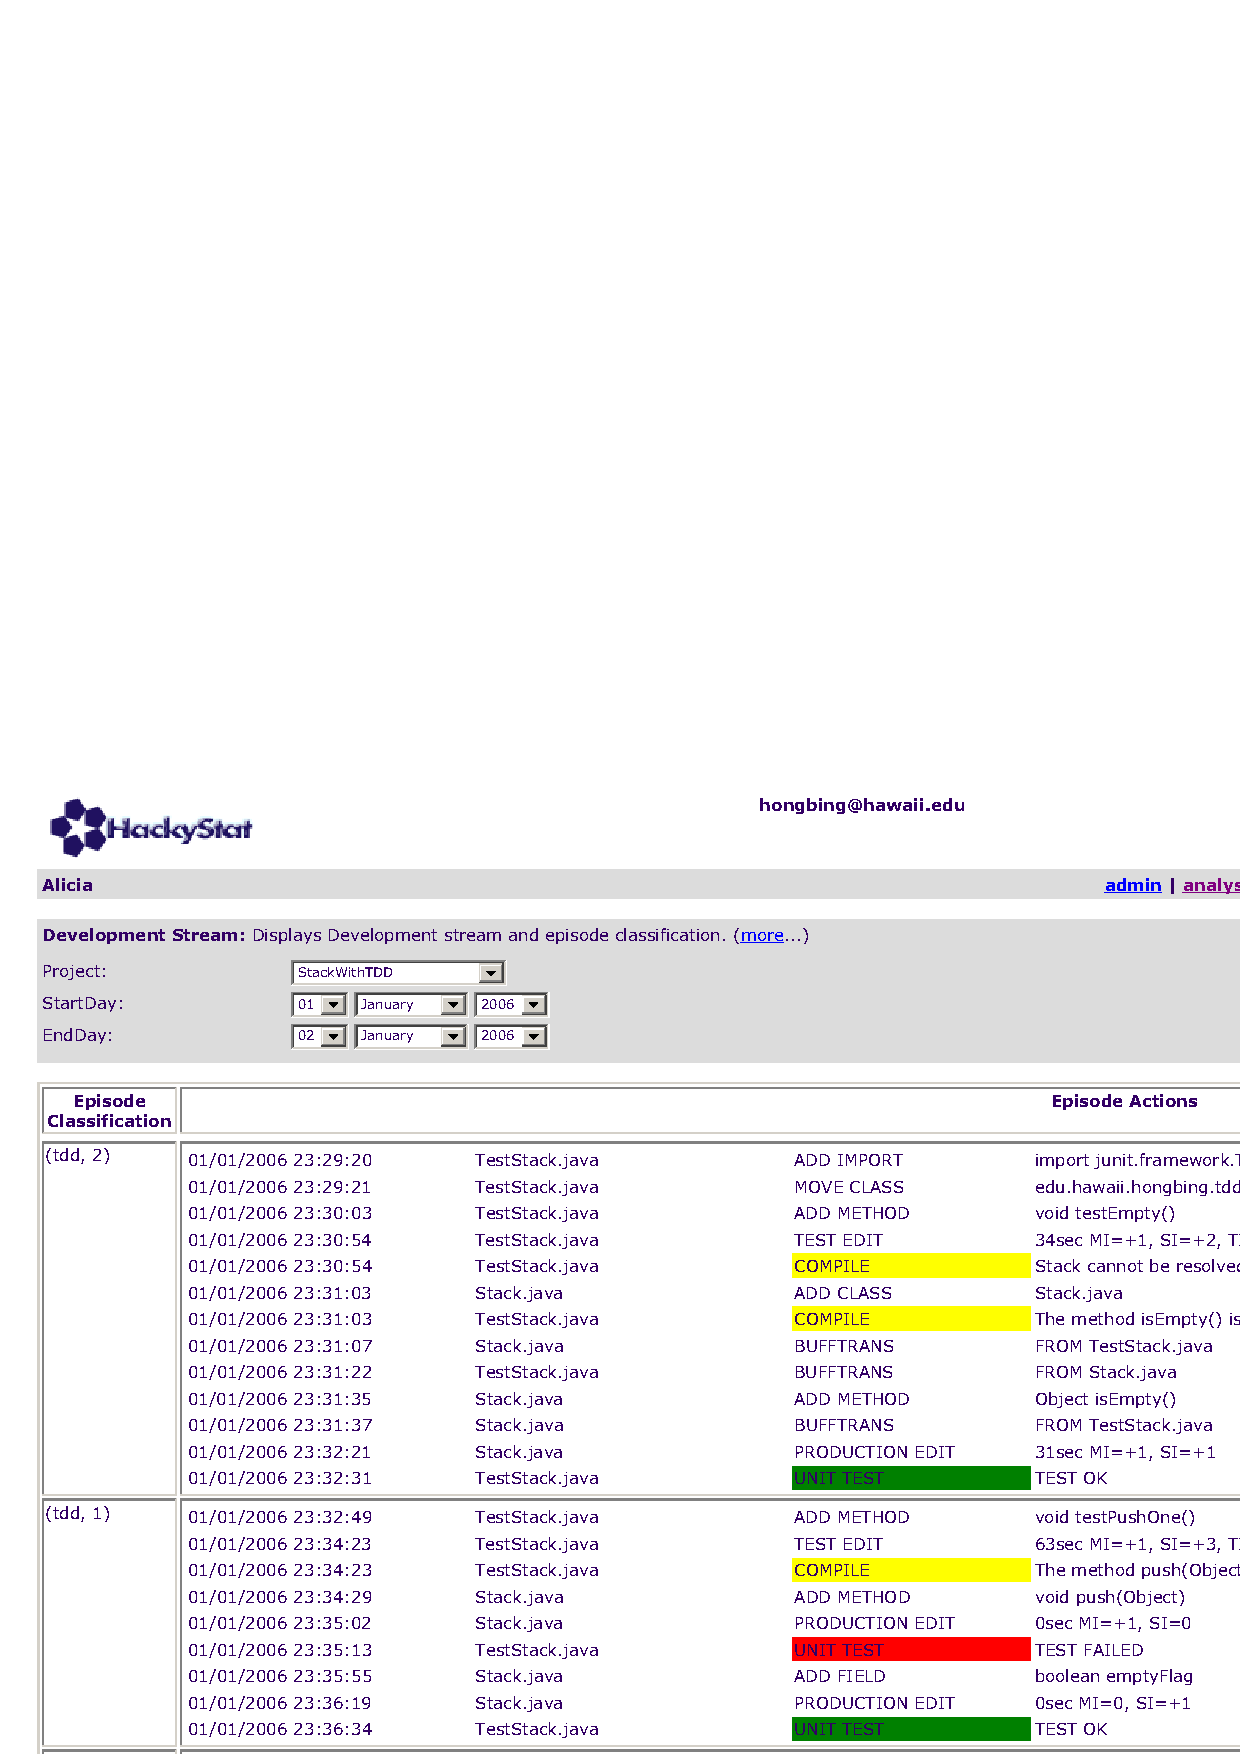
\includegraphics[width=1.0\textwidth]{figs/Zorro-Gui}
  \caption{Zorro's TDD Behavior Interface Report}\label{fig:gui}
\end{figure}

\begin{table}[htbp]
\centering
  \caption{Zorro's Inference Result Summary for Pilot Study}\label{tab:ZorroPilotStudy}  
  \begin{tabular}{|r|r|r|r|r|r|r|}
  \hline
    Subject ID & Duration & Episode & TDD & Refactoring & Test-Last & Unclassified \\ \hline
    1 & 44:53 & 15 &  6 &  1 &  7 & 1 \\ \hline
    2 & 28:17 & 13 &  5 &  0 &  8 & 0 \\ \hline
    3 & 48:00 & 14 &  9 &  0 &  5 & 0 \\ \hline
    4 & 66:32 & 14 &  5 &  1 &  8 & 0 \\ \hline
    5 & 43:14 & 16 &  3 &  1 &  7 & 5 \\ \hline
    6 & 45:57 & 11 &  4 &  0 &  7 & 0 \\ \hline
    7 & 32:40 &  9 &  4 &  1 &  3 & 0 \\ \hline \hline
    Total &   & 92 & 36 &  4 & 45 & 6 \\ 
  \hline
  \end{tabular}
\end{table}
Table \ref{tab:ZorroPilotStudy} is a brief summary of participants'
TDD behaviors inferred by Zorro. They spent 28-45 minutes for this
study and yielded 92 episodes. Zorro recognized 86 of them, which
accounts for 93.6\% of all episodes. Interestingly, among 6
unrecognizable episodes, 5 of them were from one participant only. It
was also notable that participants almost never refactored, and they
did ``Test-Last'' half of the time (in the unit of episode number).
Here ``Test-Last'' means that participants write test code after
production code has been implemented, which is the opposite side of
TDD.

\subsubsection{Development Process Video Analysis}
While participants developed solutions to the stack data structure,
they enabled ESR to record the development process as well. Here ESR
is the method for field participant observation. It captures the
Eclipse screen per second and compress the captured pictures into a
QuickTime movie file. Figure \ref{fig:EsrVideo} is a screen dump I made 
\begin{figure}[htbp]
  \centering
  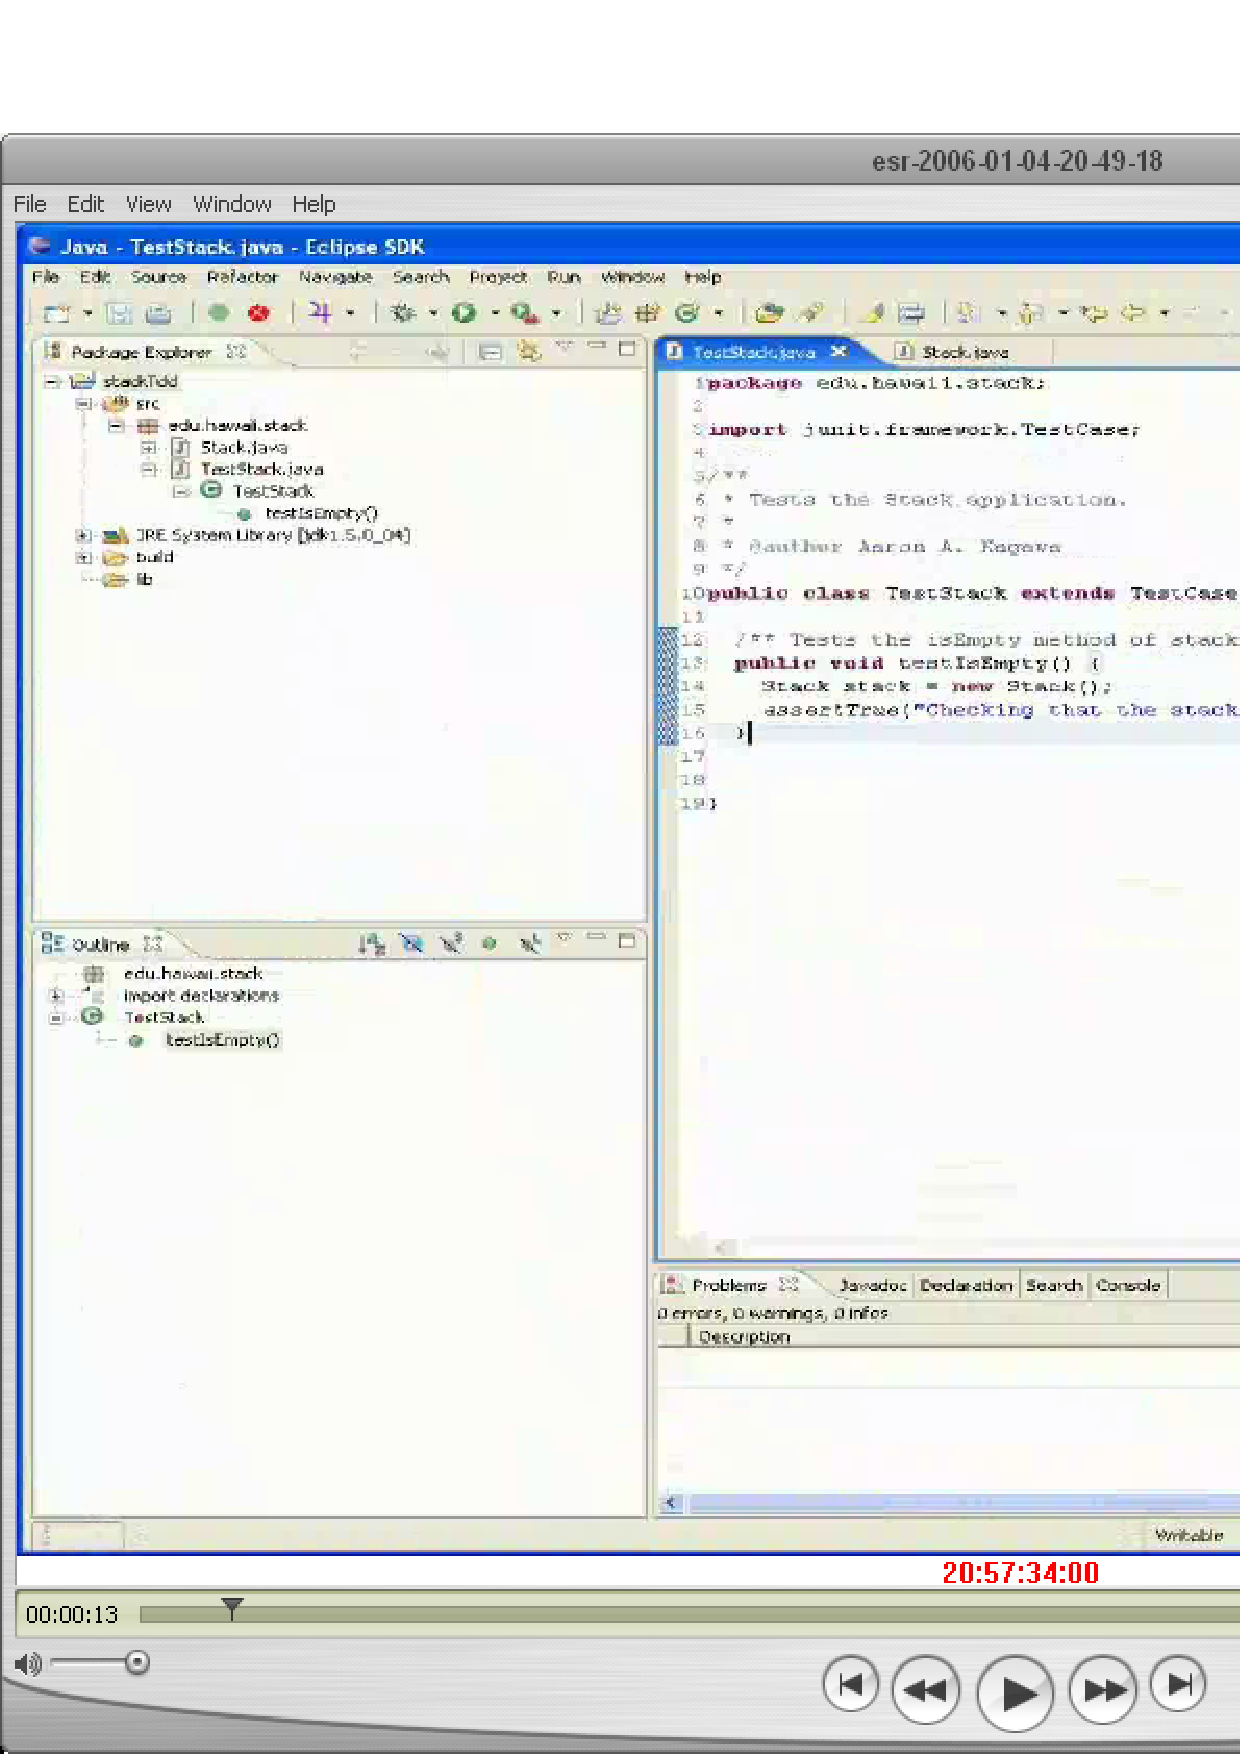
\includegraphics[width=1.0\textwidth]{figs/ESR-Video}
  \caption{Development Process QuickTime Video Recorded by ESR}\label{fig:EsrVideo}
\end{figure}
when I played and analyzed a ESR video using the QuickTime Pro software
\cite{QuickTime}.

I used Microsoft Excel for development video annotation analysis. When
there was one development activity in the recorded video, I wrote down
an entry into Excel. Each entry has the start time, end time, activity
abstract, and annotation observed from the video in Figure
\ref{fig:EsrVideoScript}.
\begin{figure}[htbp]
  \centering
  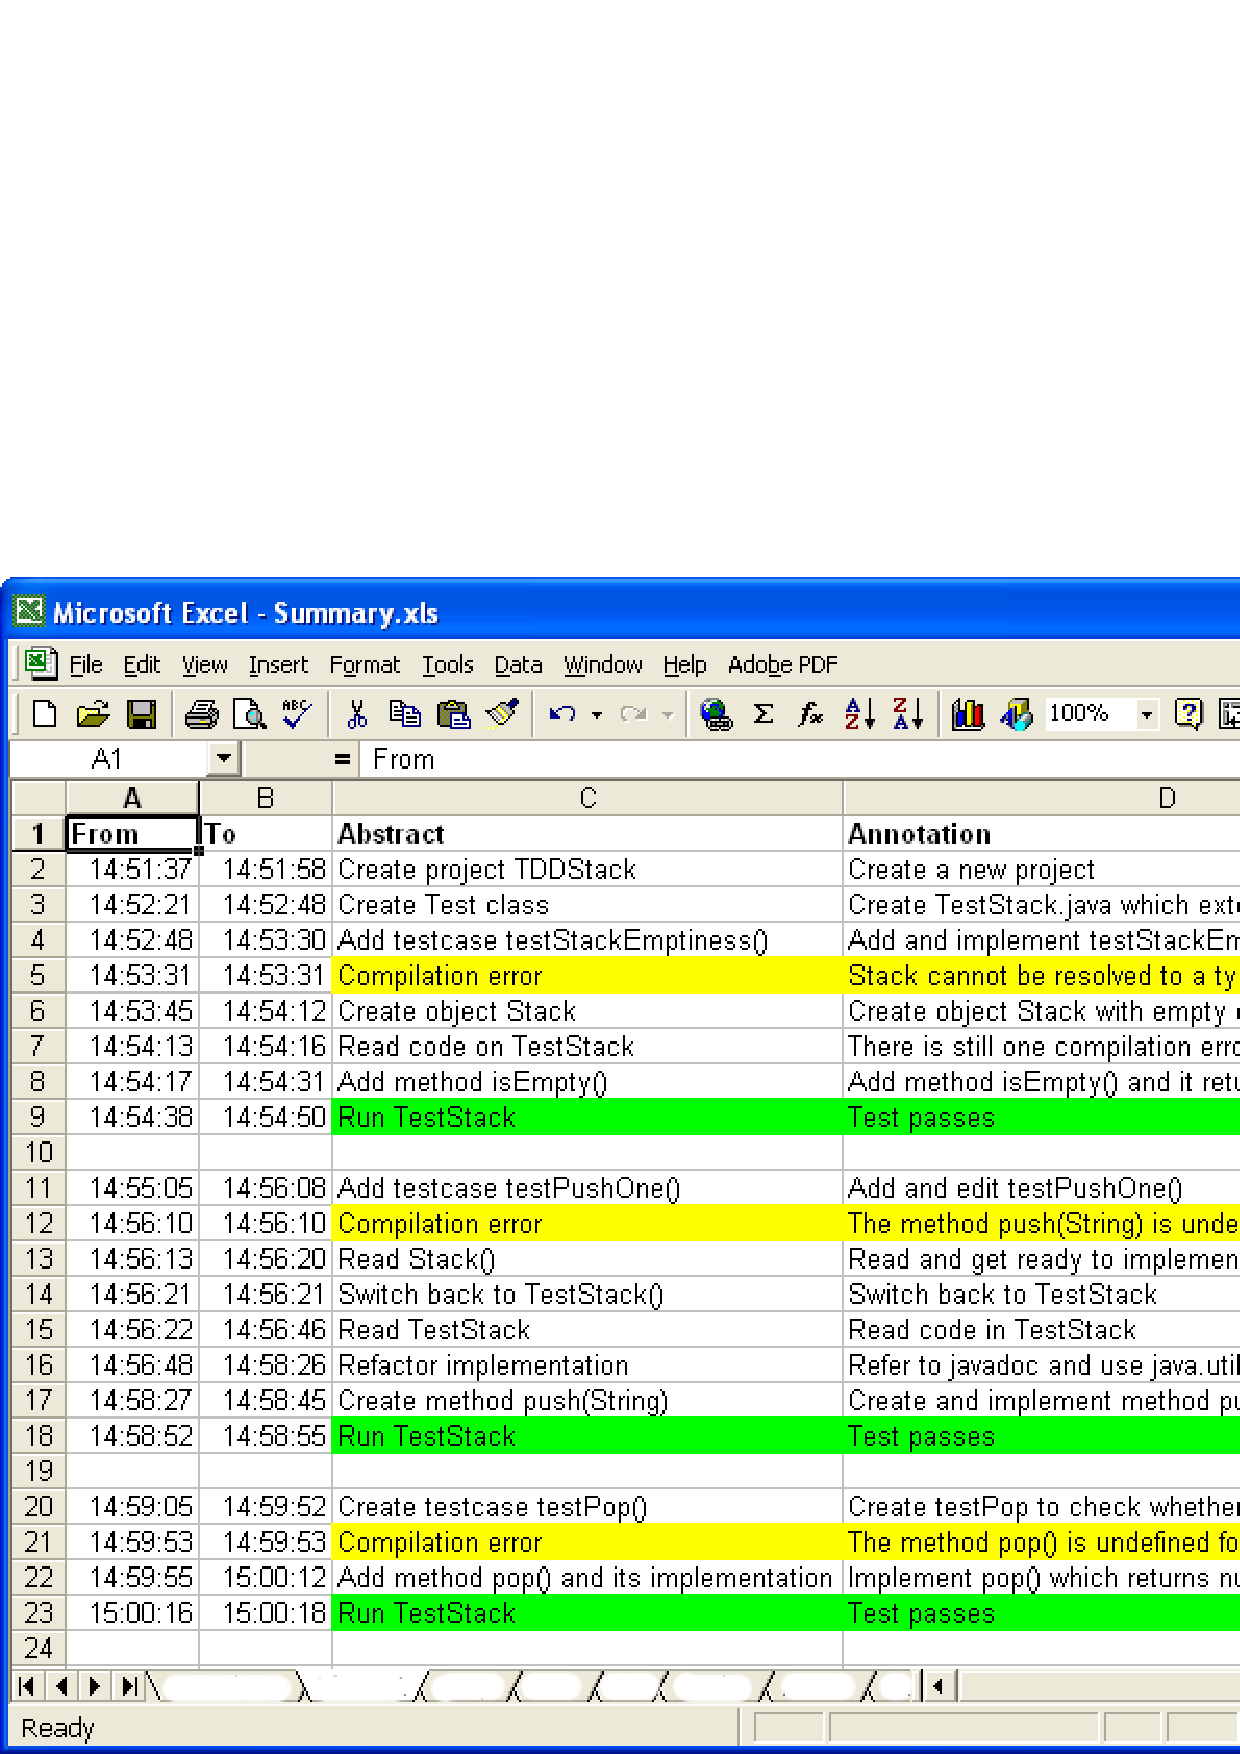
\includegraphics[width=1.0\textwidth]{figs/ESR-VideoScript}
  \caption{Development Process QuickTime Video Recorded by ESR}\label{fig:EsrVideoScript}
\end{figure}

\subsubsection{Validating Zorro's Data Collection}
The observed activities from ESR videos in Figure
\ref{fig:EsrVideoScript} were used to validate Zorro's data collection. The
comparison between the observed activities using ESR video and
activities collected by Zorro allowed us to learn: which activities
were missed by Zorro, which activities were not collected correctly,
and whether the errors were severe or not (Figure
\ref{fig:DataVerification}). In this pilot study, I found 3 types of
data collection problems in total:
\begin{itemize}
\item \textbf{Problem 1}: Edit work is not significant. 
  \begin{tabular}{lp{10cm}}
   Severity: &  \small\textit{High}\\
   Reason:   &  \small\textit{Edit work does not change object metrics: 
                         number of statements and number of methods, 
                         or there is only one state change event
                         occurred for the edit work.} \\ 
   Result:    & \small\textit{Episodes were misclassified.} \\ 
   Resolution: & \small\textit{Change the implementation of file edit 
                           sub stream in SDSA to look for file size 
                           change as well.} \\ 
   Affected: &  \small\textit{6 episodes.}
  \end{tabular}

\item \textbf{Problem 2}: Missing compilation error on test code.
  \begin{tabular}{lp{10cm}}
    Severity: & \small\textit{Low}\\
    Reason:   & \small\textit{Changes on production code cause 
                exception on inactive test code.} \\
    Results: & \small\textit{Episode were misclassified.} \\
    Resolution: & \small\textit{Fix Hackystat sensor to report all 
                  compilation on inactive file as well.}\\
    Affected: & \small\textit{2 episodes}
  \end{tabular}

\item \textbf{Problem 3}: Two unit test invocations are grouped
together or one test invocation is divided into two continuous
episodes.
  \begin{tabular}{lp{10cm}}
    Severity: & \small\textit{Medium}\\
    Reason: & \small\textit{Eclipse sensor collects multiple data 
              entries for one invocation.}\\
    Results: & \small\textit{Two or more episodes were grouped 
               together or divided resulting that they cannot be 
               classified correctly.} \\
    Resolution: & \small\textit{Tag one unit test invocation with run 
                  time to group multiple unit test entries belong to 
                  one test invocation together.} \\
    Affected: & \small\textit{3 episodes}
  \end{tabular}
\end{itemize}

\noindent Note that these errors affected 11 episodes in this study. 

\subsubsection{Validating Zorro's TDD Behavior Inference}
ESR was the method we used to observe the participants' behaviors. By
playing the recorded movie file, I compared the observed behaviors to
the participants' TDD behaviors inferred by Zorro. Table
\ref{tab:EsrPilotStudy} lists the comparison results.
\begin{table}[htbp]
\centering
  \caption{Validation Result by ESR Video Analysis for Pilot Study}\label{tab:EsrPilotStudy}  
  \begin{tabular}{|r|r|r|r|r|r|r|}
  \hline
    Subject ID & Episode & Classified & Wrongly Classified & Percentage \\ \hline
    1          & 15 &  14 &  2 & 13.3\% \\ \hline
    2          & 13 &  13 &  3 & 23.3\% \\ \hline
    3          & 14 &  14 &  1 &  7.1\% \\ \hline
    4          & 14 &  14 &  1 &  7.1\% \\ \hline
    5          & 16 &  11 &  1 &  9.1\% \\ \hline
    6          & 11 &  11 &  1 &  9.1\% \\ \hline
    7          &  9 &   9 &  1 & 12.5\% \\ \hline \hline
    Total      & 92 &  86 & 10 & 11.6\% \\ 
  \hline
  \end{tabular}
\end{table}
This manual comparison by human being concluded that 11.6\% of the
recognized episodes were wrongly inferred by Zorro in this study. It
indicates that Zorro infers developer's TDD behaviors correctly 88.4\%
of the time.

Data collection problems caused most of the inference errors.
Infrequent invocation of unit testing by participants was another
problem, which yielded episodes with too many activities. Problem 4
describes this type of error.
\begin{itemize}
\item {\textbf{Problem 4}: An episode has too many activities.
  \begin{tabular}{lp{10cm}}
    Severity: & \small\textit{Low}\\
    Reason: & \small\textit{Participants did not invoke unit testing 
              frequently enough.}\\
    Results: & \small\textit{Episodes were misclassified.}\\
    Resolution: & \small\textit{Introduce long episode type and 
                  avoid inferring episode with too many activities.} \\ 
    Affected: & \small\textit{2 episodes}
  \end{tabular}}
\end{itemize}

\subsection{Conclusion and Discussion}

Participants in this study spent 28 to 66 minutes on the
programming task using TDD. Zorro partitioned the overall development
efforts into 92 episodes, out of which 86 were classifiable; 6 were
unclassifiable. It classified 76 out of 86 episodes correctly
resulting in classification accuracy rate 88.4\%.

The analysis result demonstrates that Zorro has the potential to 
understand developer's TDD development behaviors automatically 
using low-level development activities. Using ESR video analysis, we
found that there were 3 kinds of data collection problems in Zorro, 
which affected 11 out of 92 episodes. Overall, it collects enough 
low-level development activities correctly most of the time for TDD 
behavior inference. This provides the supporting evidence to research 
question Q1a. Following this study, I fixed these three data
collection problems in the current version of Zorro.

Two out of 93 episodes were incorrectly inferred by Zorro because its
inference rules do not work well for long episodes which have too many
activities internally. It provides the supporting evidence to research
question Q1b. In the current version of Zorro, I improved the
inference rule for relatively long episodes, and introduced a new type
of episodes which have too many activities or lasts too long a time.

The results from this pilot study indicates that the research method is
appropriate. The ESR has the capability to record incremental small
changes made by participants. Although ESR caused a small delay
when it is initialized, participants did not notice much
delay in the development process. With the ESR video, I was able to
validate both the Zorro's data collection and inferences of TDD
behavior. Thus, there is supporting evidence to research question
Q1c. The ESR is an appropriate tool to observe participant's
programming behaviors for Zorro validation study.

Overall, Zorro works well in collecting low-level development
activities and inferring developer's TDD behaviors in the pilot
study. However, one problem with our pilot study is that participants
only spent 50\% of their development time doing TDD. There are several
possibilities that could explain this phenomenon. One possibility
could be that stack is too simple and developers did not need to fail
tests first to have the correct implementation. Or it could be that
Beck's concise summary of TDD is just too simple. Real TDD
development is much more complicated than he described. For instance,
a developer can add a new test that does not fail initially because
the functional code works well even without any change. This
development pattern should be TDD compliant although it is neither
test-driven nor refactoring. Therefore, I defined a more sophisticated
two-step model to infer TDD development behaviors (Figure
\ref{fig:heuristic}) in this study.
\begin{figure}[htbp]
  \centering
  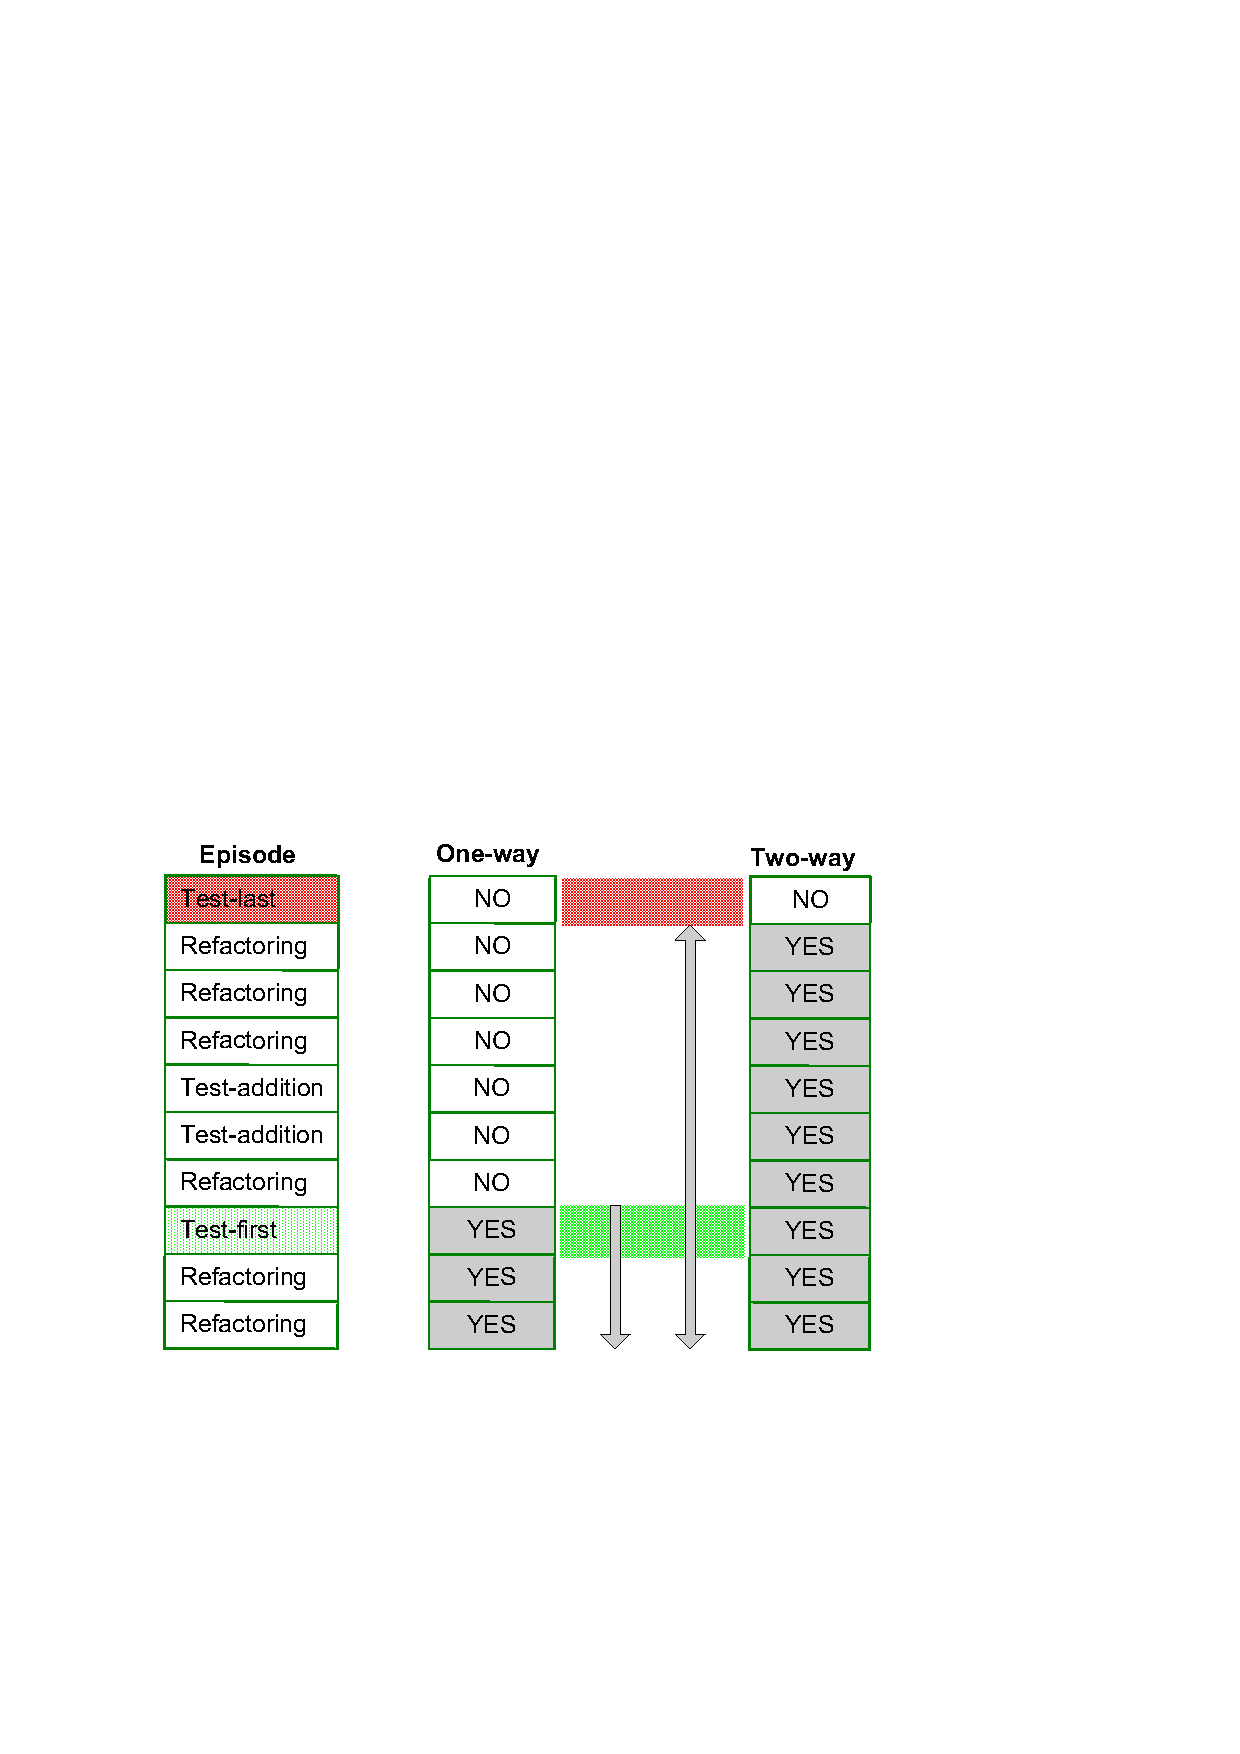
\includegraphics[width=0.8\textwidth]{figs/HeuristicAlgorithms}
  \caption{TDD Heuristic Algorithms}\label{fig:heuristic}
\end{figure}
First, TDD development episodes are classified independently using
internal data. Second, a heuristic algorithm is applied to determine
whether an episode is TDD conformant or not. Figure
\ref{fig:heuristic} has three lists. The left-most one is a list of
episodes recognized by Zorro's TDD inference rules. As their names
indicate, the episodes can be ``test-first", ``test-addition",
``refactoring", or ``test-last" etc. The one-way and two-way TDD
heuristic algorithms are on the right side of Figure
\ref{fig:heuristic}. The one-way algorithm uses look-forward approach
to determine whether an episode is TDD conformant, while the two-way
heuristic algorithm uses both look-forward and look-backward
approaches. Figure \ref{fig:heuristic} indicates this difference using
a single-head arrow and a double-head arrow. Our preliminary work suggests 
that the two-way heuristic algorithm can understand real world situations
better than the one-way algorithm.

\subsection{Validity Analysis}
There were several threats to the validity of this study. One of them
is that some participants did not know TDD well prior to the
study. Therefore, we provided a graphic illustration of the TDD rhythm
\cite{TDDRhythm} and a short list of TDD reference guides
\cite{TDDQuickReference}.  Another threat to validity is that certain
applications are hard to test. To minimize the effects of
untestability, we used the simple and well-known stack problem in this
study. With regard to the validity of data collection, we used
unobtrusive data collection utilities: the Hackystat Eclipse Sensor
and ESR. Both tools required little overhead from participants
\cite{csdl2-03-12,Hackystat} at the beginning or end of the study.

There were two valid external validity problems in this study. The
first one was the simplicity and stringency of TDD. In the pilot
study, we interpreted TDD as strictly as Kent suggested in
\cite{Beck:01,Beck:03} and Doshi recommended in
\cite{TDDRhythm,TDDQuickReference}. The second one was that we only
had 7 participants in this study. We hope to address both problems in
the future studies.

\section{Zorro Validation Case Study}
The pilot study of Zorro was a success. It convinces us that Zorro's
rule-based approach has promise for developer's TDD behavior
inference. It also demonstrates that the research methodology works.
Following this study, I fixed several data collection problems found
in the pilot study. We also improved Zorro's TDD inference rules
based on the pilot study and collaboration with Software
Engineering Group at the National Research Council of Canada.

In Fall 2006, we plan to conduct a case study of Zorro in a software
engineering class at the University of Hawaii.

\subsection{Purpose of the Study}
Currently Zorro collects development activity data more accurately,
has a more sophisticated episode classification schema, and infers
developer TDD behaviors based not only on the episode's internal
structure but also the context in which the episode occurred.
The purpose of this study is to:
\begin{enumerate}
\item perform Zorro validation study using the Eclipse Screen Recorder;
\item perform a second type of validation in which participates
provide feedback through the web-based validation wizard of Zorro;
\item obtain feedback regarding whether Zorro can help TDD
beginners through a post-test interview.
\end{enumerate}

\subsection{Research Questions}
In this case study I will test Zorro's abilities to: collect the
necessary activity data, infer TDD behaviors correctly, and help
beginning TDD learners. The specific research questions for this study
are:

\begin{itemize}
\item{Q2a: Does Zorro collect software development activities
accurately enough for episode partitioning and TDD behavior
inference?}
\item{Q2b: Does Zorro's inference of TDD behaviors agree with
analyses based upon participant observation?}
\item{Q2c: Does Zorro's inference of TDD behaviors agree with what
participants believe to be their TDD behaviors?}
\item{Q2d: Does Zorro provide useful information for beginners to
understand TDD and improve their TDD development?}
\end{itemize}

Note that these research questions support the overall research
questions for this thesis as described in Chapter
\ref{ch:researchquestions}.

\subsection{Research Methodology and Design}
\subsubsection{Participants}
The participants in this study will be students in the software
engineering classes at the University of Hawaii during Fall 2006. Unit
testing and Test-Driven Development are two skills required by this
study. There are 15-16 students in this class and we anticipate that
at least a dozen students will participate in this study.

\subsubsection{Design and Experimental Manipulation}
This study uses mixed research methods\cite{Creswell:03}. While test
subjects work on the bowling game problem using TDD, we will record
their development process with ESR\cite{esr}. After finishing the TDD
programming, participants will launch the analysis validation wizard
of Zorro to validate its TDD behavior inference. Finally, we will
interview them. The study will last 2 hours for each test subject
including a 90-minute TDD programming session, a 15-minute Zorro
evaluation session, and a 15-minute interview.

\subsubsection{Instruments}
Eclipse is the IDE that will be used. We will instrument participants'
TDD development using the Hackystat Eclipse sensor\cite{SensorInstall}
and ESR\cite{esr}. Participants will evaluate Zorro's inference of
their TDD development using Zorro's web validation wizard. We will
also record the participant interview with notepad and tape recorder.

\subsubsection{Procedure}
Students will learn TDD in the software engineering class and have
hands-on practice on TDD programming after the class. After this
training, we will request volunteers to participate this case study,
and schedule a 2 hour time slot to participate the study in the lab.
There, they will do TDD development on the ``bowling score keeper''
problem (Appendix \ref{app:UserStoriesBSK}) for 90 minutes. Afterwards we
will ask them to validate Zorro's inferences of their TDD
development. Finally I will interview them for 15 minutes. Below is a
more detailed description of this case study procedure.

\begin{enumerate}
\item{Teaching of TDD}

Instructor of the software engineering class will give a TDD lecture
to students. Students will have the first 20 pages of \cite{Beck:03}
as the reading assignment and a hands-on practice on ``Roman Numeral'' as the
programming assignment.

The lecture will include the following contents:
\begin{itemize}
\item Introduction to TDD
  \begin{itemize}
  \item The two principles of TDD from \cite{Beck:03}
  \item The red/green/refactor pattern of TDD
  \item TDD rhythm \cite{TDDRhythm}
  \item TDD vs. Unit Testing
  \item A TDD example: implementing stack by writing test first 
  \end{itemize}
\item Why TDD?
  \begin{itemize}
    \item{Developer gets quick feedback.}
    \item{TDD improves software quality.}
    \item{TDD promotes simple design.}
    \item{Microsoft has successful story on TDD \cite{Bhat:06}}
    \item{Test Driven Development proves useful at Google\cite{RoyOsheroveBlog}}
  \end{itemize}
\item About TDD
  \begin{itemize}
    \item{TDD may not be appropriate for everybody.}
    \item{TDD is about design.}
    \item{Some studies show that TDD improves software quality.}
    \item{TDD may reduce productivity.}
    \item{TDD references including testdriven.com, mailing list and blogs.}
  \end{itemize}
\item Reading and programming assignments
  \begin{itemize}
    \item {Page 1-20 of Beck's book ``Test-Driven Development by Example'' \cite{Beck:03}}
    \item {TDD Quick Reference \cite{TDDQuickReference}}
    \item {Practice TDD on Roman Numeral Problem (Appendix
    \ref{app:UserStoriesRomanNumeral})}
  \end{itemize}
\end{itemize}

\item{TDD Development in the Lab (90 minutes)}

``Bowling score keeper" is a widely used problem for TDD research. I
designed user stories for this problem to fit the purpose of this case
study research. Participants will develop solutions following the
provided user stories (Appendix \ref{app:UserStoriesBSK}). A 90-minute time
limit will be enforced. This time frame should be sufficient
regardless whether they finish the programming task or not.

\item{Zorro's TDD Behavior Inference Validation (15 minutes)}

After participants finish the TDD programming work on the bowling
game, they will use the Zorro evaluation wizard to analyze their TDD
development and validate Zorro's TDD behavior inference (Figure
\ref{fig:EpisodeFeedback}).

\item{Interview (15 minutes)}

In the end I will interview participants. The purpose of this
interview is to learn participant's opinions on unit testing and TDD,
discover questions and problems they may have, and investigate whether and
how Zorro can help TDD beginners. The interview protocol and outline
are available at Appendix \ref{app:CaseStudyInterviewGuide}.

\end{enumerate}

\subsubsection{Data Collection}
Hackystat sensor data and the participants' Zorro evaluations will 
be stored at the remote Hackystat server. ESR will record the TDD 
development process into QuickTime movie files in the lab computers. 
In the interview I will use notepad and tape recorder to record 
the conversations with participants.

\begin{comment}
\subsection{Validity Analysis}
A challenging task of this study is to let all participants install
ESR and enable it in their development processes. As in other behavior
related research, recording development activities is challenging
because participants may have privacy concerns. Therefore, we will
state that participating this study will not affect their grades. And
we will not disclose their identities in the analysis and report of
this study (see the consent form in Appendix \ref{app:CaseStudyConsentForm}).

In order to generalize Zorro's TDD episode inference accuracy
regarding hypothesis 2, we estimate sample size requirement according
to \cite{Cochran:77}. The analysis unit is episode, and we select
confidence level 95\%. To be statistically important, we will need
138~245 episodes. Since we may have 12 participants in this study, it
will be enough if every participant contributes 20 or more TDD
development episodes. A recent dry-run test revealed that one test
subject can yield 23 episodes.
\end{comment}

\subsection{Proposed Data Analyses}
\subsubsection{Zorro Data Collection Validation}
The Hackystat Eclipse sensor collects low-level development activities.
These raw sensor data are sent to a Hackystat server. Zorro processes
these raw sensor data to perform TDD behavior inference. One purpose
of this analysis is to verify that the Hackystat Eclipse sensor can
collect enough development activity data, and collect it correctly for
TDD developer behavior inference.  There are two aspects of this
problem. One aspect is whether collected data are accurate, which
is research question Q2a. The other aspect is whether the data
collection errors will cause episode misclassification, which is
related to research questions Q2a and Q2b.

I will use the same analysis method as in the pilot study. First, I
will play the development process video recorded by ESR to observe the
development activities. Then I will write down the observed
development activities into Excel as shown in Figure
\ref{fig:VideoExcel}.
\begin{figure}[htbp]
  \centering
  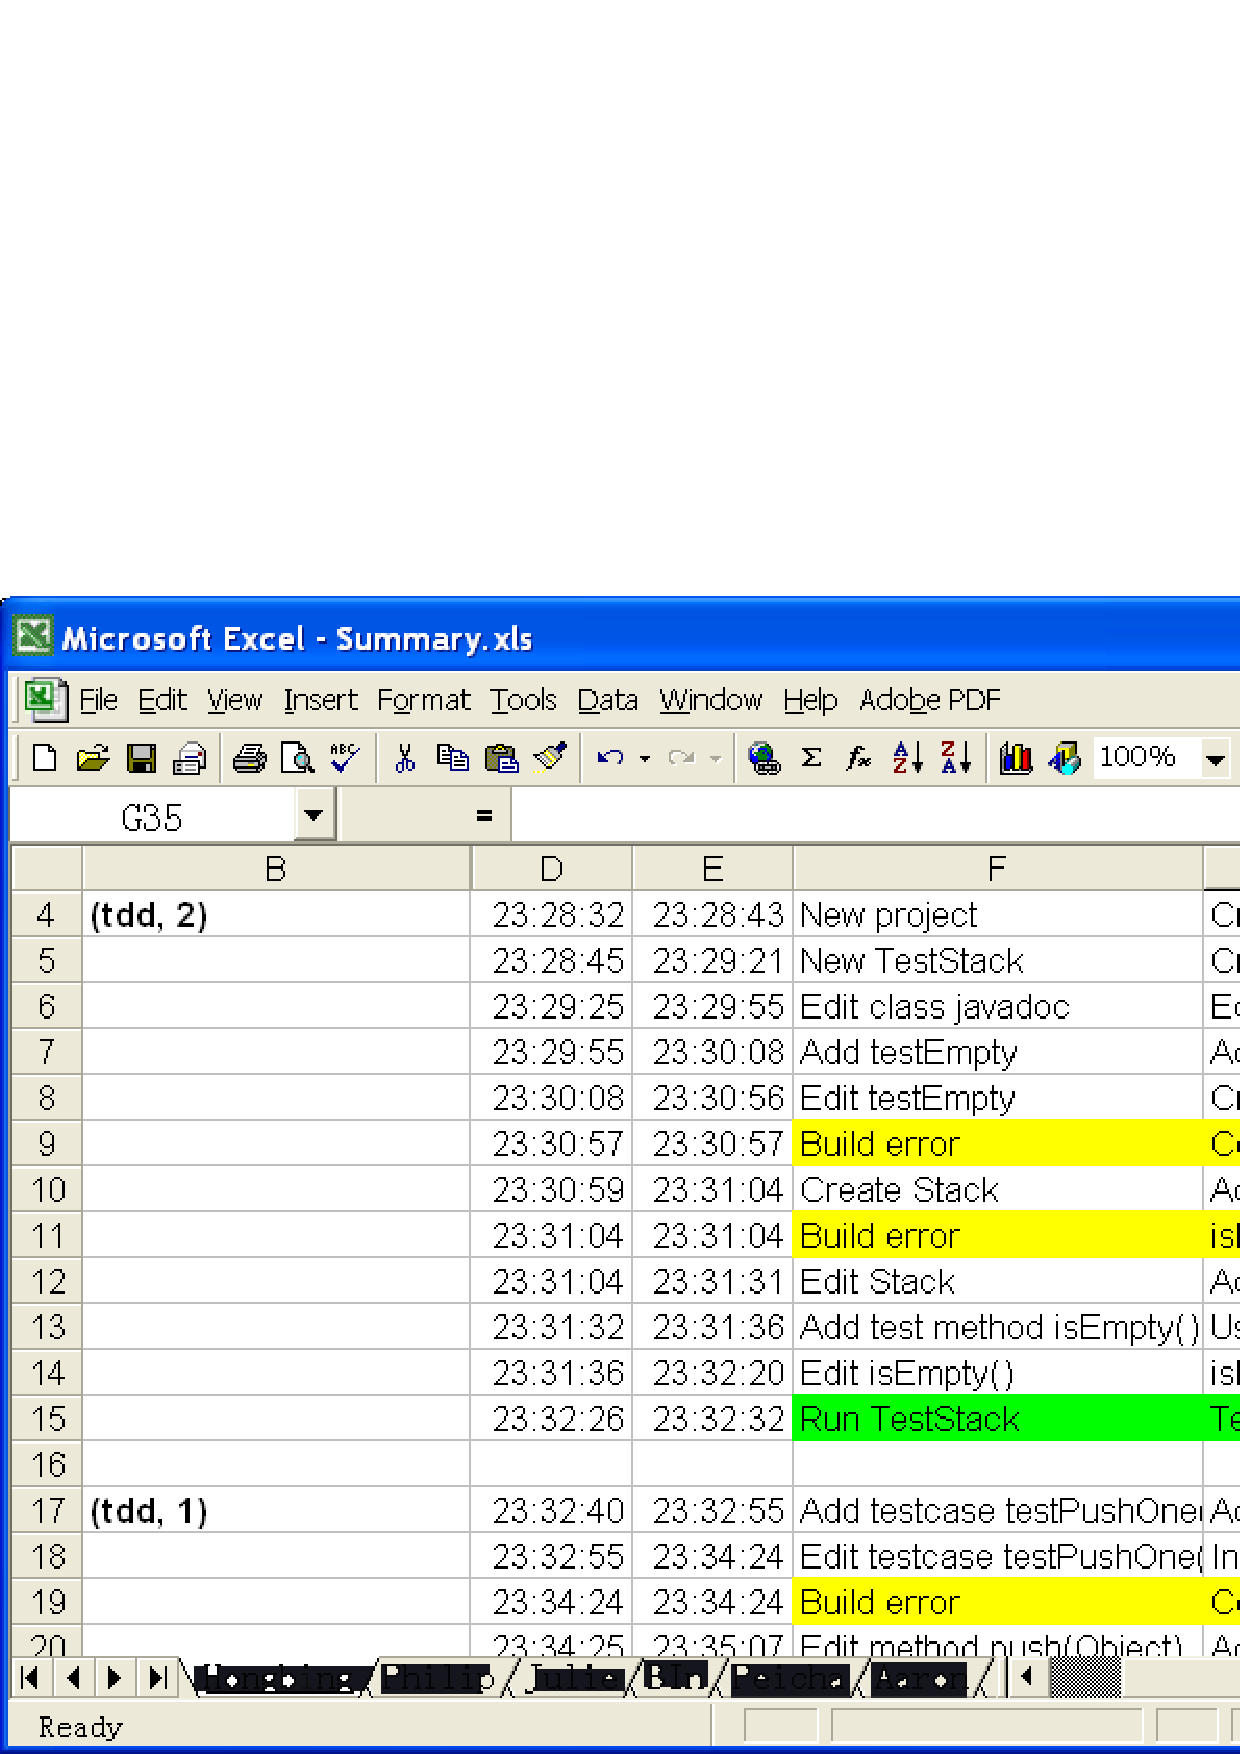
\includegraphics[width=1.0\textwidth]{figs/VideoScriptExcel}
  \caption{Example of ESR Video Script}\label{fig:VideoExcel}
\end{figure}

The observed development activities are used for comparison against the
development activities reduced by Zorro (Figure \ref{fig:gui}) from
raw sensor data. Figure \ref{fig:DataVerification} is an excerpt of the
comparison of the development activities from these two data
sources. Comparing the two sources of data will allow us to verify
Zorro's data collection completeness and correctness.
\begin{figure}[hbtp]  
\centering
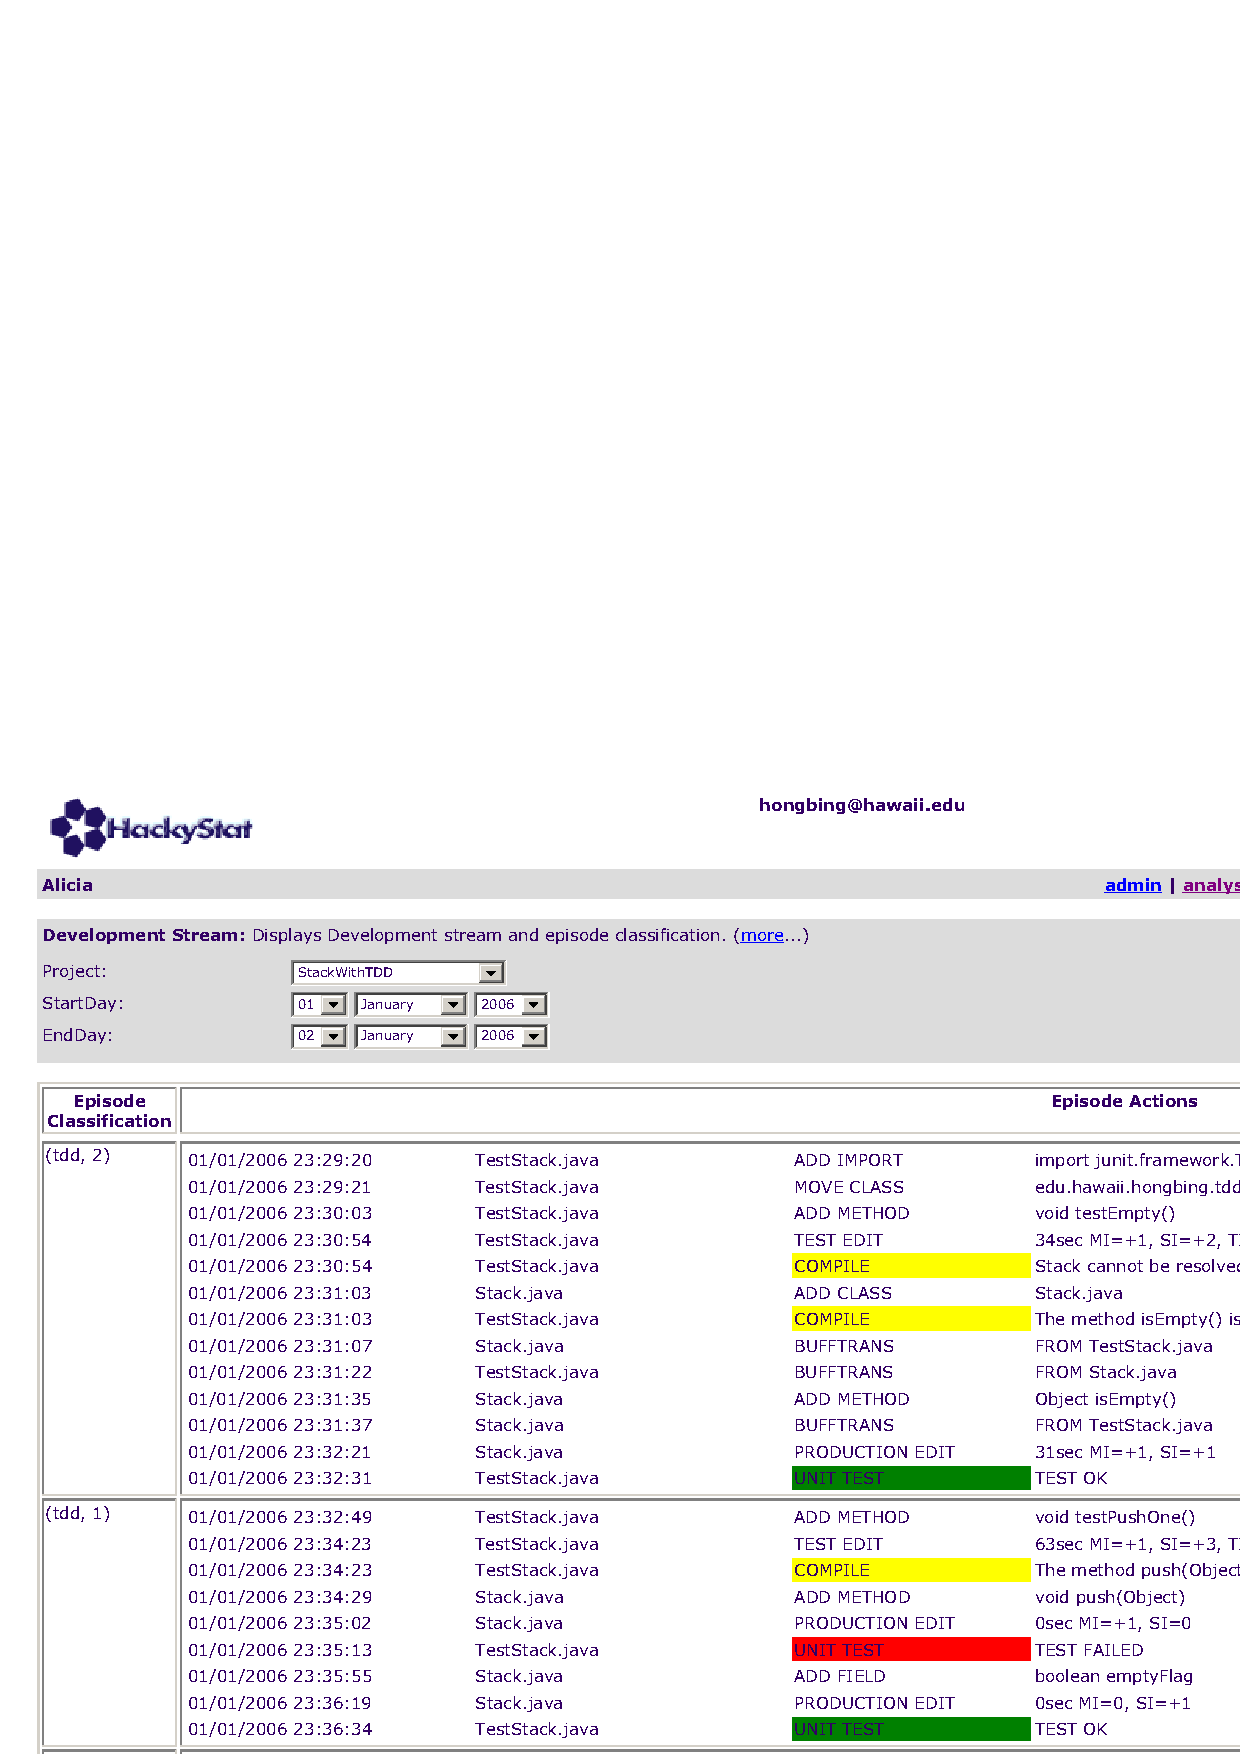
\includegraphics[width=0.48\textwidth]{figs/Zorro-Gui} 
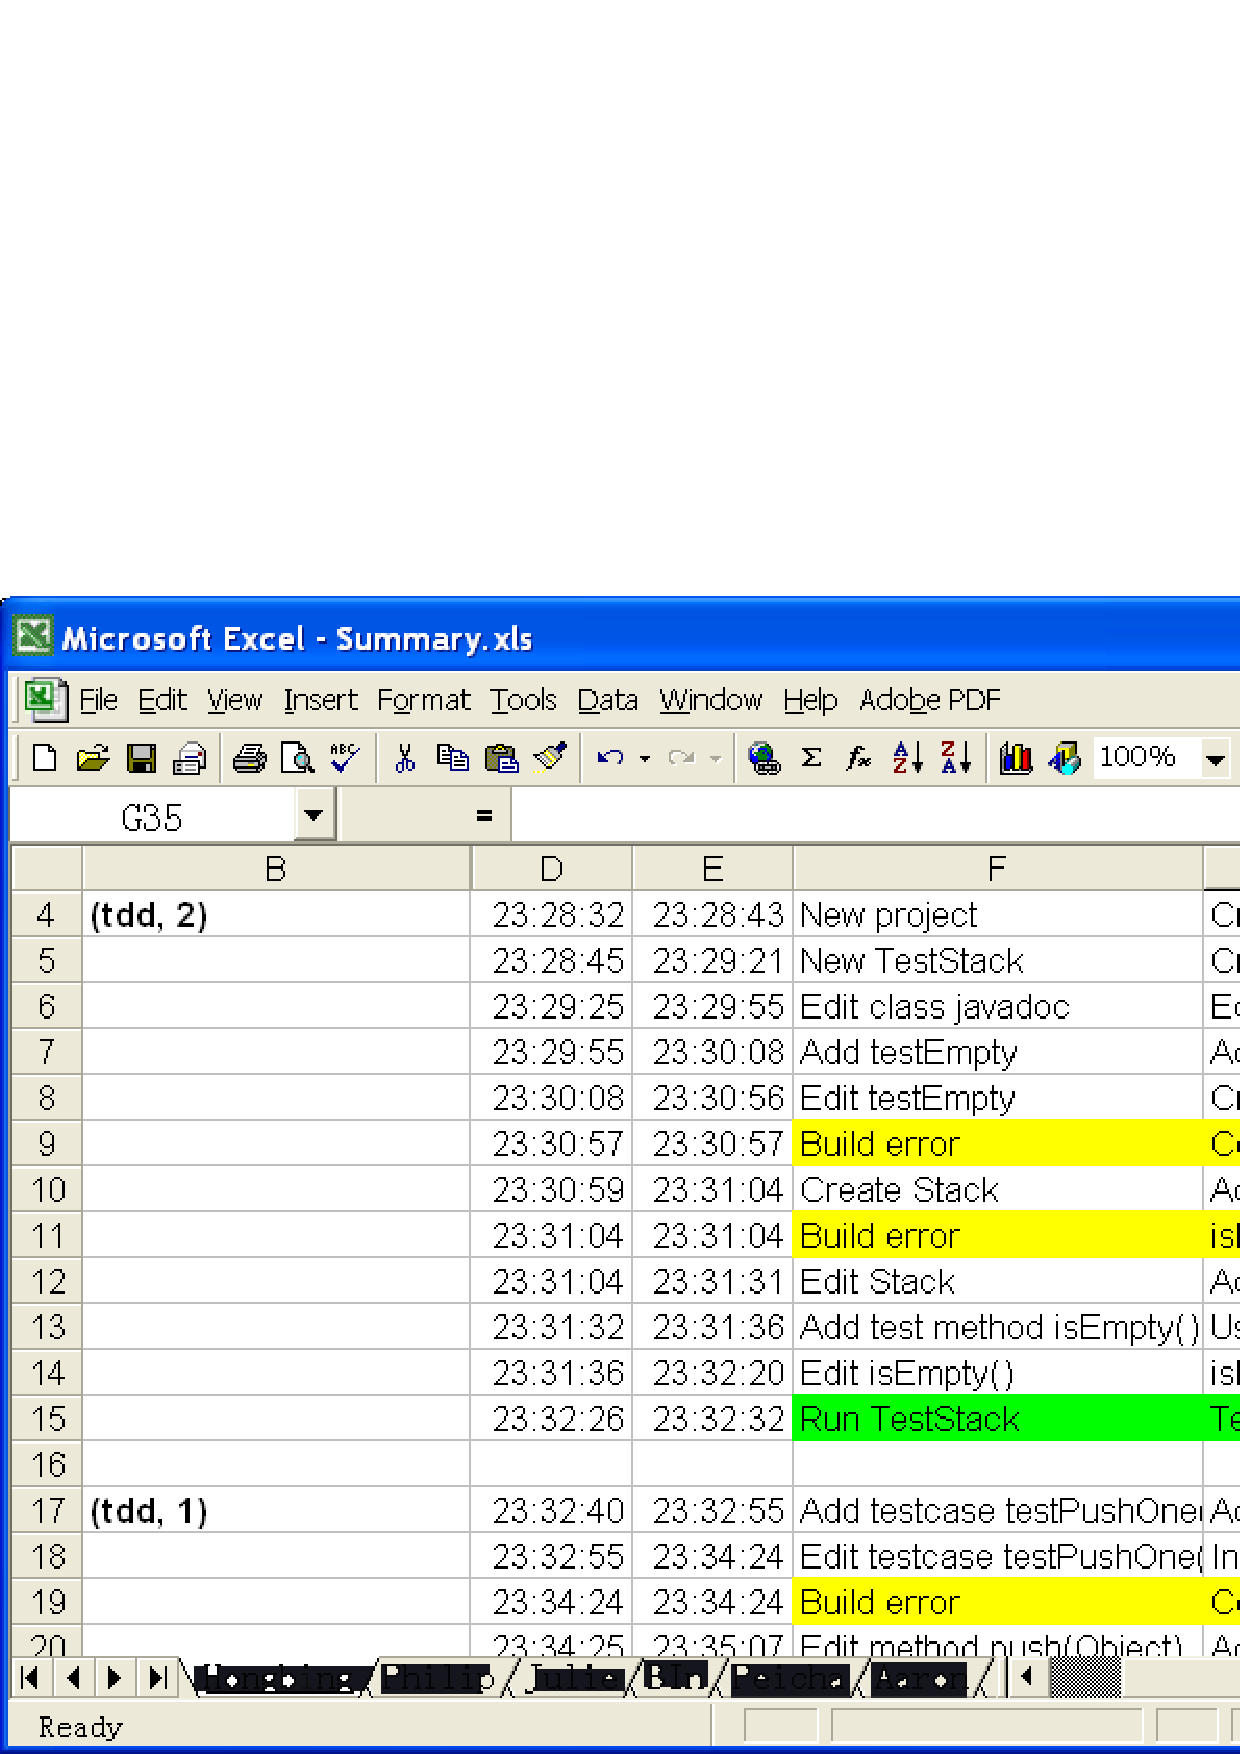
\includegraphics[width=0.48\textwidth]{figs/VideoScriptExcel}
\caption{Example of Development Activity Comparison between Zorro and
ESR}
\label{fig:DataVerification}
\end{figure}

I will use the descriptive analysis to summarize analysis results
after comparing the two data sources. For example, assuming there is a
problem in collecting unit test invocations, I will present it as
follows:
\begin{itemize}
\item \textbf{Problem}: Two unit test invocations are grouped together.
\item \textbf{Result}: Two or more episodes can be grouped together so 
that they cannot be classified correctly.
\item \textbf{Affected Episodes}: 2
\end{itemize}

\subsubsection{Validating Zorro's TDD Behavior Inference}
The purpose of this analysis is to answer research question Q2b, that
is, whether Zorro's TDD behavior inference agrees with the observed
behaviors of the participants using ESR. ESR video is the method used
for participant observation in this study. As in the pilot study, we
will use the ESR video to validate Zorro's TDD behavior inference. By
playing the movie files produced by ESR, we can observe the
participants' development behaviors (Figure
\ref{fig:VideoZorroComparison}).
\begin{figure}[htbp]
  \centering
  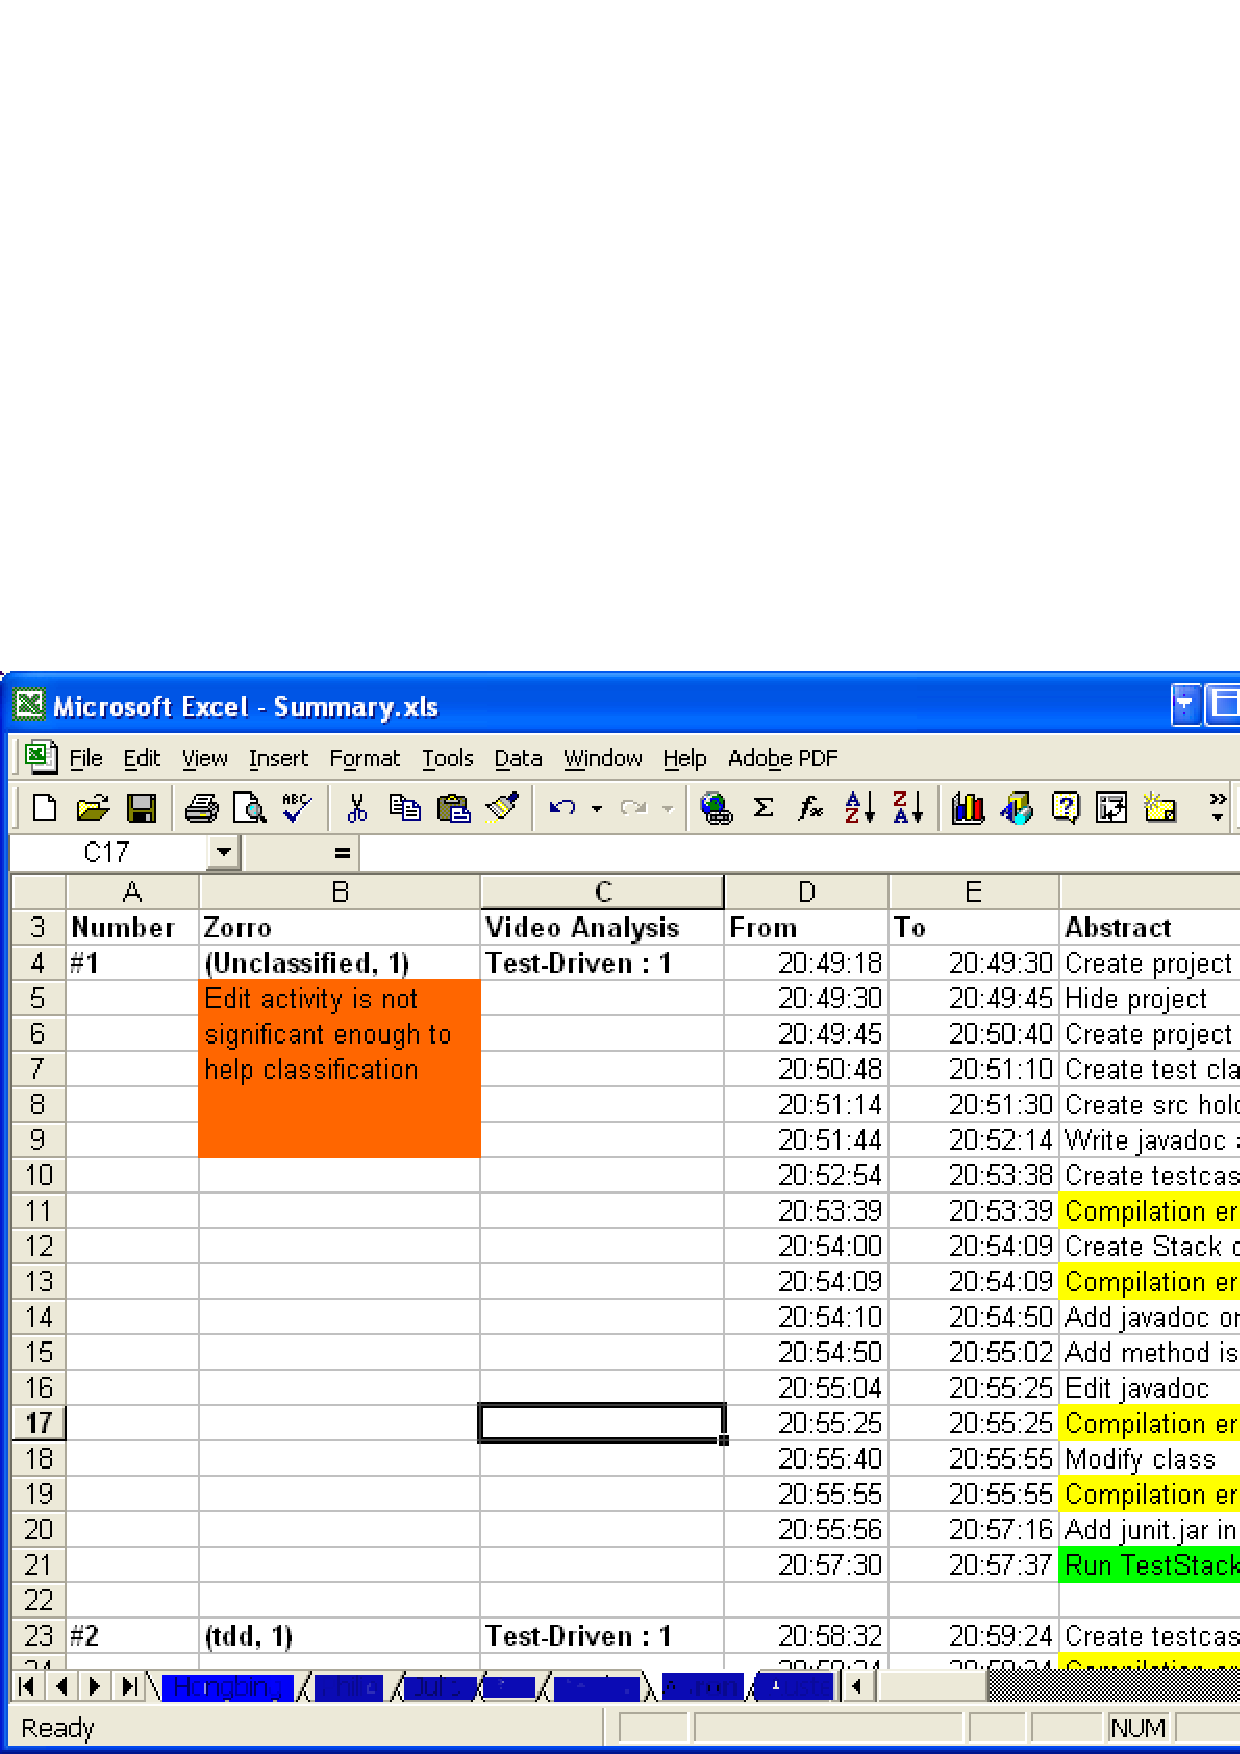
\includegraphics[width=0.65\textwidth]{figs/VideoZorroComparison}
  \caption{Example of Development Behavior Observed via ESR}\label{fig:VideoZorroComparison}
\end{figure}
For example, in the programming session Figure
\ref{fig:VideoZorroComparison}, Zorro failed to recognize a legitimate
TDD development behavior because the inference rules were
insufficient. I will use a table as shown in Table
\ref{tab:EpisodeValidationSummary} to summarize the episode validation results.
\begin{table}[htbp]
\centering
  \caption{Example of TDD Episode Validation Results}\label{tab:EpisodeValidationSummary}  
  \begin{tabular}{|r|r|r|r|r|r|}
  \hline
    Subject & Duration & Finished & Total & Correctly Recognized & Inference\\ 
    ID &  & User Stories & Episodes & Episode & Accuracy \\ \hline
    1 & 44:53 & 10 & 15 & 15 & 100\% \\ \hline
    2 & 28:17 & 13 & 20 & 19 & 95\% \\ \hline
    3 & 48:00 & 8 & 14 & 13 & 93\% \\ \hline
    4 & 66:32 & 12 & 20 & 18 & 90\% \\ \hline
    5 & 43:14 & 11 & 22 & 22 & 100\% \\ \hline
    6 & 45:57 &  9 & 15 & 13 & 87\% \\
  \hline
  \end{tabular}
\end{table}

\subsubsection{Using Developer's Feedback as a Second Method for Zorro Validation}
TDD is a new practice aiming at ``clean code that
works''. Red/green/refactor is Beck's simple model of TDD; however, it
may be too simple for real world situations. For example, experienced
TDD developers often write a series of tests that do not require
additional production code implementation. In Zorro, I developed a set
of rules to infer developer's TDD behavior based on Beck's TDD
principle and additional knowledge from TDD practitioners. Therefore,
Zorro's TDD inference is somewhat subjective.  The purpose of this
analysis is to provide additional data from participants to
cross-validate Zorro's TDD behavior inference. This effort supplies 
research question Q2-4, that is, whether participants agree with
Zorro's TDD developer behavior inference.

Zorro provides an episode validation analysis for users. This analysis
presents Zorro's TDD behavior inference and the underlying reasoning
process. It provides three choices for participants to indicate whether
they agree or not with Zorro's inference on their TDD development
behaviors. In the same analysis, they can also use a set of check-boxes
and a text-box to provide additional information about their actual 
development behaviors (Figure \ref{fig:EpisodeFeedback}).
\begin{figure}[htbp]
  \centering
  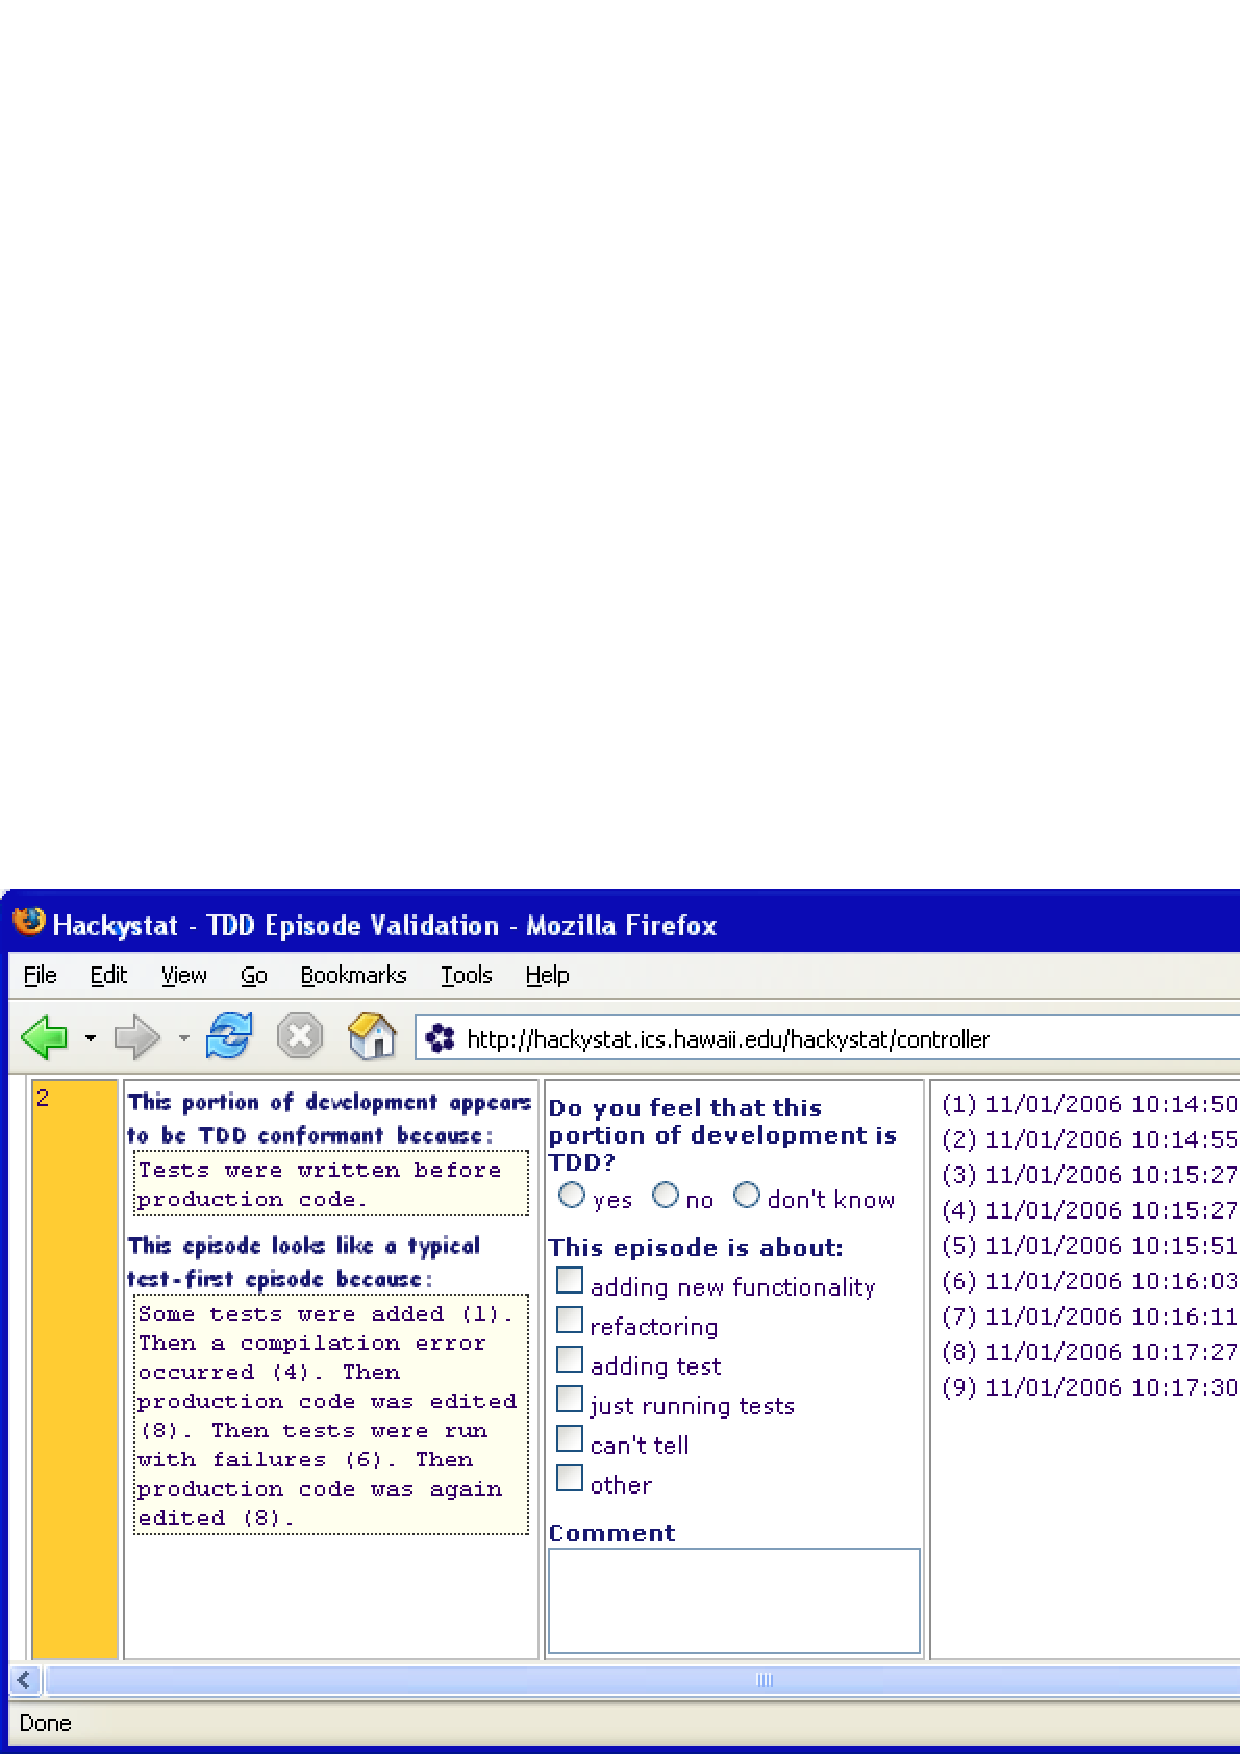
\includegraphics[width=1.0\textwidth]{figs/EpisodeFeedback}
  \caption{Episode Feedback}\label{fig:EpisodeFeedback}
\end{figure}

This analysis cross-validate the TDD behavior validation analysis using
ESR video. I will use tables \ref{tab:TDDEpisodeFeedbackSum} and
\ref{tab:NonTDDEpisodeFeedbackSum} to report the analysis results.
\begin{table}[htbp]
\centering
  \caption{Example of TDD Episode Feedback Summary}\label{tab:TDDEpisodeFeedbackSum}  
  \begin{tabular}{|r|r||r|r|r|r|}
  \hline
    Subject ID & Episodes & TDD Episodes & Episodes agreed & Episodes disagreed & Unsure \\ \hline
    1 & 20 & 18 & 16 & 1 & 1 \\ \hline
    2 & 14 & 14 & 14 & 0 & 0 \\ \hline
    3 & 19 & 15 & 15 & 0 & 0 \\ \hline
    4 & 24 & 20 & 19 & 0 & 1 \\ \hline
    5 & 22 & 22 & 22 & 0 & 0 \\
  \hline
  \end{tabular}
\end{table}
\begin{table}[htbp]
\centering
  \caption{Example of Non-TDD Episode Feedback Summary}\label{tab:NonTDDEpisodeFeedbackSum}  
  \begin{tabular}{|r|r||r|r|r|r|}
  \hline
    Subject ID & Episodes & Non-TDD Episodes & Episodes agreed & Episodes disagreed & Unsure \\ \hline
    1 & 20 & 2 & 1 & 0 & 1 \\ \hline
    2 & 14 & 0 & 0 & 0 & 0 \\ \hline
    3 & 19 & 4 & 3 & 1 & 0 \\ \hline
    4 & 24 & 4 & 4 & 0 & 0 \\ \hline
    5 & 22 & 0 & 0 & 0 & 0 \\
  \hline
  \end{tabular}
\end{table}
I will employ categorization and description to interpret the research
findings. Tables \ref{tab:TDDEpisodeFeedbackSum} and
\ref{tab:NonTDDEpisodeFeedbackSum} illustrate the summary of this analysis.

\subsubsection{Analysis of Participant Interviews}
The purpose of this analysis is to answer research question Q2-4, that
is, whether Zorro provides useful information for TDD beginners. I
will use the interview research method to collect data about:
participant's opinions on unit testing and TDD, Zorro's usefulness,
and whether Zorro is helpful for TDD beginners. I will put
participants in two categories according to their opinions on unit
testing: developers who are strongly in favor of unit testing for high
quality software, and those who are not. Since TDD depends on unit
testing, this categorization will help us understand TDD beginners'
needs better.

In the interview, I will ask participants to evaluate the usefulness
of Zorro's 5 TDD analyses. If an analysis is useful, then I will ask
what it can be used for. I will use the pattern matching analytic
technique to summarize the interview data. For example, participants
who are enthusiastic about TDD improvement may find the ``Zorro
Demography Analysis'' to be very helpful for them. The participants
who do not buy into TDD may only want to know whether their manager
will be okay with their TDD performance if it is required.

\begin{comment}
\subsubsection{Zorro usefulness study}
We will conduct pretest and posttests surveys to investigate
participants' perceptions of TDD and how can Zorro change their
perceptions of TDD after using it. Participants' feedbacks on Zorro's
TDD episode inferences will be used to interpret the differences
between pretest and posttest. Thus, we will use two means to justify
our answer to research question Q4. That is, to what extents, do
participants agree on Zorro's inferences of their TDD development?
\subsection{Anticipated Results}
To some degree, this study is a replication of the previous pilot
study, but we will extend this study to include more participants and
use a web-based validation approach. For research questions Q1-Q3, we
expect more accurate low-level development data collection and more
accurate TDD episode inference. Since students' expertise on TDD is
limited, we can foresee that the web-based validation may not give us
enough information, but we can use this opportunity to fine-tune
Zorro's web-based validation method.
\end{comment}

\section{External Case Study}
The pilot study and case study are the foundations of this research
for evaluating the automation of TDD behavior inference. This last study 
complements the previous studies by gathering feedback from the 
community of TDD practitioners and researchers.

\subsection{Purpose of the study} 
The first two studies tested the capabilities of Zorro's TDD behavior
inference in laboratory environments.  The
purpose of this study is to:
\begin{itemize}
\item validate Zorro's rule-based inference of developer's TDD behaviors;
\item investigate Zorro's uses for TDD learning, improvement, and research.
\end{itemize}

\subsection{Research Questions}
The specific questions for this research are:
\begin{itemize}
\item Question Q3a: Does Zorro infer the TDD behaviors correctly as
participants' perception?
\item Question Q3b: Are Zorro's TDD analyses useful for participants?
\item Question Q3c: How can Zorro be used to assist TDD learning,
improvement, or research?
\end{itemize}

\subsection{Research Methodology and Design}
\subsubsection{Participants}
The participants of this study will be TDD learners, practitioners,
and researchers from the TDD community. We will solicit participation 
from the TDD community using email and news group.

\subsubsection{Design and Experimental Manipulation}
This external case study will use the one-shot case study research
method. Zorro will be the treatment of this study. We will collaborate
with participants evaluating Zorro in their environments. We will
interview the participants to collect data. 

\subsubsection{Procedure}
\begin{enumerate}
\item Zorro Demo Implementation 

As a first step, I implemented a demonstration wizard of Zorro
showing the capabilities of Zorro \cite{ZorroDemo:06}. This
application demonstrates 5 analyses Zorro provides, each comes with
the introduction and interesting findings. The demo also provides a
feedback page for viewers to reach us.

\item Participation Invitation

We will disseminate an email with the description and purpose of this
study to the community of empirical software researchers and XP
practitioners. The future actions will depend on what feedback we will
get.
\end{enumerate}